\documentclass{beamer}
\mode<presentation>
{
	\usetheme{Frankfurt}
	\setbeamercovered{transparent}
}

\usepackage[russian]{babel}
\usepackage[utf8x]{inputenc}
\usepackage{listings,bera}
\lstset{language=Python, numberstyle=\tiny, keywordstyle=\color{blue},numbers=left,commentstyle=\color{green},
basicstyle=\footnotesize}

\usepackage{mathptmx}
\usepackage{graphics}
\usepackage[scaled=.90]{helvet}
\usepackage{courier}
\usepackage[T1]{fontenc}

\title{Development and Debugging of Information Measurement and Control
Systems for Mobile Robots with Python Dynamic Language}
\author{Kirsanov K.B.}
\institute[sensorika]
{Keldysh Institute of Applied Mathematics RAS, Sensorika lab}
\date{26.11.09 / DAAAM 2009 | Section C3: Algorithms}

\beamerdefaultoverlayspecification{<+->}

\begin{document}

\begin{frame}
\titlepage
\end{frame}

\begin{frame}
\frametitle{Contents}
\tableofcontents
\end{frame}

\section{Introdution}

\subsection{Robotics Develompemt Kits(RDK) }
\begin{frame}
\frametitle{RDK}
\framsubetitle{Robotics Develompemt Kits:}
\begin{itemize}
\item<1> \textbf{Microsoft Robotics Studio} \textit{http://msdn.microsoft.com/en-us/robotics/default.aspx}
\item<1> \textbf{Player Project} \textit{http://playerstage.sourceforge.net}
\item<1> \textbf{ORCA2} \textit{http://orca-robotics.sourceforge.net/orca/index.html}
\item<1> \textbf{LAAS/GenoM} \textit{https://softs.laas.fr/openrobots/wiki/genom}
\item<1> \textbf{Marie} \textit{http://marie.sourceforge.net}
\item<1> \textbf{URBI} \textit{http://www.urbiforge.com}
\item<1> \textbf{Webots} \textit{http://www.cyberbotics.com}
\item<1> \textbf{RoboJRE} \textit{http://www.ridgesoft.com/robojde/robojde.htm}
\item<1> \textbf{OROCOS} \textit{http://www.orocos.org}
\end{itemize}
\end{frame}

\subsection{How does they work?}
\begin{frame}
\frametitle{How does they work?}
\begin{itemize}
	\item<1>\textbf{Main} development language: С, С++, Java, C\#
	\item<1>'Multi-agent approach' (System are composed of multiple interacting agents like engine, sensor, camera, etc.).
	\item<1>This agents interacts via RPC (Remote Procedure Call) abstraction.
\end{itemize}
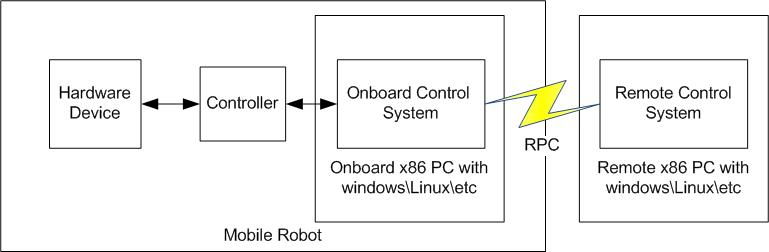
\includegraphics[width=10.5cm]{rpc0.jpg}
\end{frame}

\subsection{Problems due development and debugging}
\begin{frame}
\frametitle{Problems:}
\framesubtitle{Real robot != model}
\begin{itemize}
\item<1>RPC implies a call for existing functions, while the development process is accompanied by their creation and
modification. Thus, there is need for continuous updating the interprocess communication protocol and on-board control 
system.
\item<1>Onboard control system implemented on a compiled language, and any update requires them to be re-compiled and
restarted;
\end{itemize}
Disadvantages: 
\begin{itemize}
\item<1>It`s hard to develop - creating and testing of new algorithms requires a fairly lengthy restart procedure 
 and greatly slows development process;
\item<1>It`s hard to debug - impossible to dynamicly update working code onboard;
\end{itemize}
\end{frame}

\section{New Approach}
\subsection{New system arcitecture}
\begin{frame}
\frametitle{New system arcitecture}
\framesubtitle{Not just another RDK or framework but new paradigm}

To overcome this difficulties we are using:
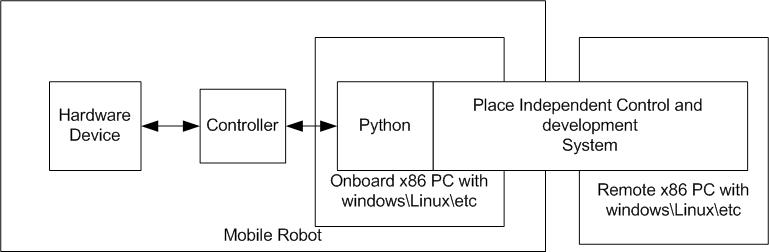
\includegraphics[width=10.5cm]{rpc1.jpg}
\begin{itemize}
 \item<1>A dynamic interpreted language Python as a base testing and development language;
 \item<1>Implemented Turing-complete protocol;
\end{itemize}
\end{frame}

\subsection{Dynamic interpreted language}
\begin{frame}
\frametitle{Dynamic interpreted language}
\framesubtitle{Program like a clay in hands of potter}
\begin{itemize}
\item<1>Language “dynamics” allows executing at runtime many behaviors that other languages might perform during compilation;
\item<1>These behaviors could include extension of the program, by adding new code, by extending objects and definitions, or by modifying the type system, 
all during program execution. This behavior used to change the behavior of control system without reboot;
\item<1>Main program can be updated in the field conditions
\end{itemize}
We can chose from Lua, Tk, Python, JS or create new one.
\end{frame}

\subsection{Turing-complete protocol}
\begin{frame}
\frametitle{Turing-complete protocol}
\begin{itemize}
\item<1>Changing the hardware component of mobile robot or mechatronic devices requires a corresponding change in control
program. As a rule, it should also change the control protocol (i.e. adding new commands, modifying or delete existing ones). The control protocol is, in fact, is a programming language, and it can be evaluated in terms of Turing completeness;
\item<1>Instead of a permanent updating (after the hardware change or new behavior implementation) the protocol, it makes sense to
immediately implement a "Turing-complete protocol.";
\item<1>This will allow to execution is not only trivial commands, but entire programs with multiple branches that, in turn,
will smear the border between developer workstation and the onboard computer;
\end{itemize}
\end{frame}

\subsection{Why Python?}
\begin{frame}
\frametitle{Why Python}
\begin{itemize}
  \item<1> It`s free and open source;
  \item<1> Minimalistic syntax helps in semi-automatic code-generation and reduces network traffic;
  \item<1> Acces to abstract syntax tree and introspection; 
  \item<1> A lot of good libraries (graphs, liner algebra, statistics, etc.);
  \item<1> Flat learning curve;  
\end{itemize}
\end{frame}

\section{Real life example: 'Smooth start'}

\begin{frame}
\frametitle{Real life example: 'Smooth start'}
\framesubtitle{\textbf{Classic RPC-style}}
Breef: A foolish robot with only one command: SetEnginePWM\footnote{PWM - Pulse-width modulation}(int PWM\_Value).
We have to start smoothly, to save engines from destruction. 

\lstinputlisting{SmoothStart.py}
Nagle's algorithm or random drops of network rate makes impossible to make a real smooth movement.
We have to stop robot, update it`s software with new command, start robot and, finally, call it. Soon our protocol will be full of
such speacial commands for special cases.
\end{frame}

\begin{frame}
\frametitle{Real life example: Smooth start}
\framesubtitle{\textbf{New coding style}}
\lstinputlisting{SmoothStart2.py}
No need to stop the robot. No need to recompile. No need to spend time on updating protocol.

\end{frame}

\section{Main results}
\begin{frame}
\frametitle{Main results:}
\begin{enumerate}
  \item<1> Development cycle time are decreased up to 3-5 times;
  \item<1> Source code size decreases up to 4-5 times;
  \item<1> The border between developer workstation and the onboard computer are smeared;
  \item<1> Plugin for Eclipse IDE
\end{enumerate}
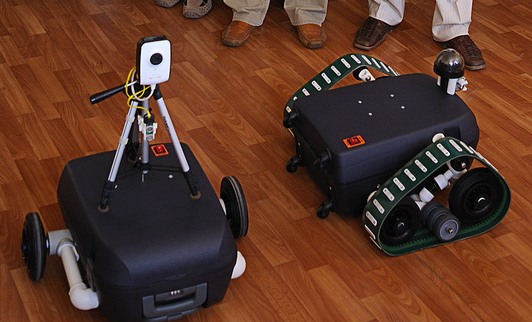
\includegraphics[width=3.2cm]{rob1.jpg}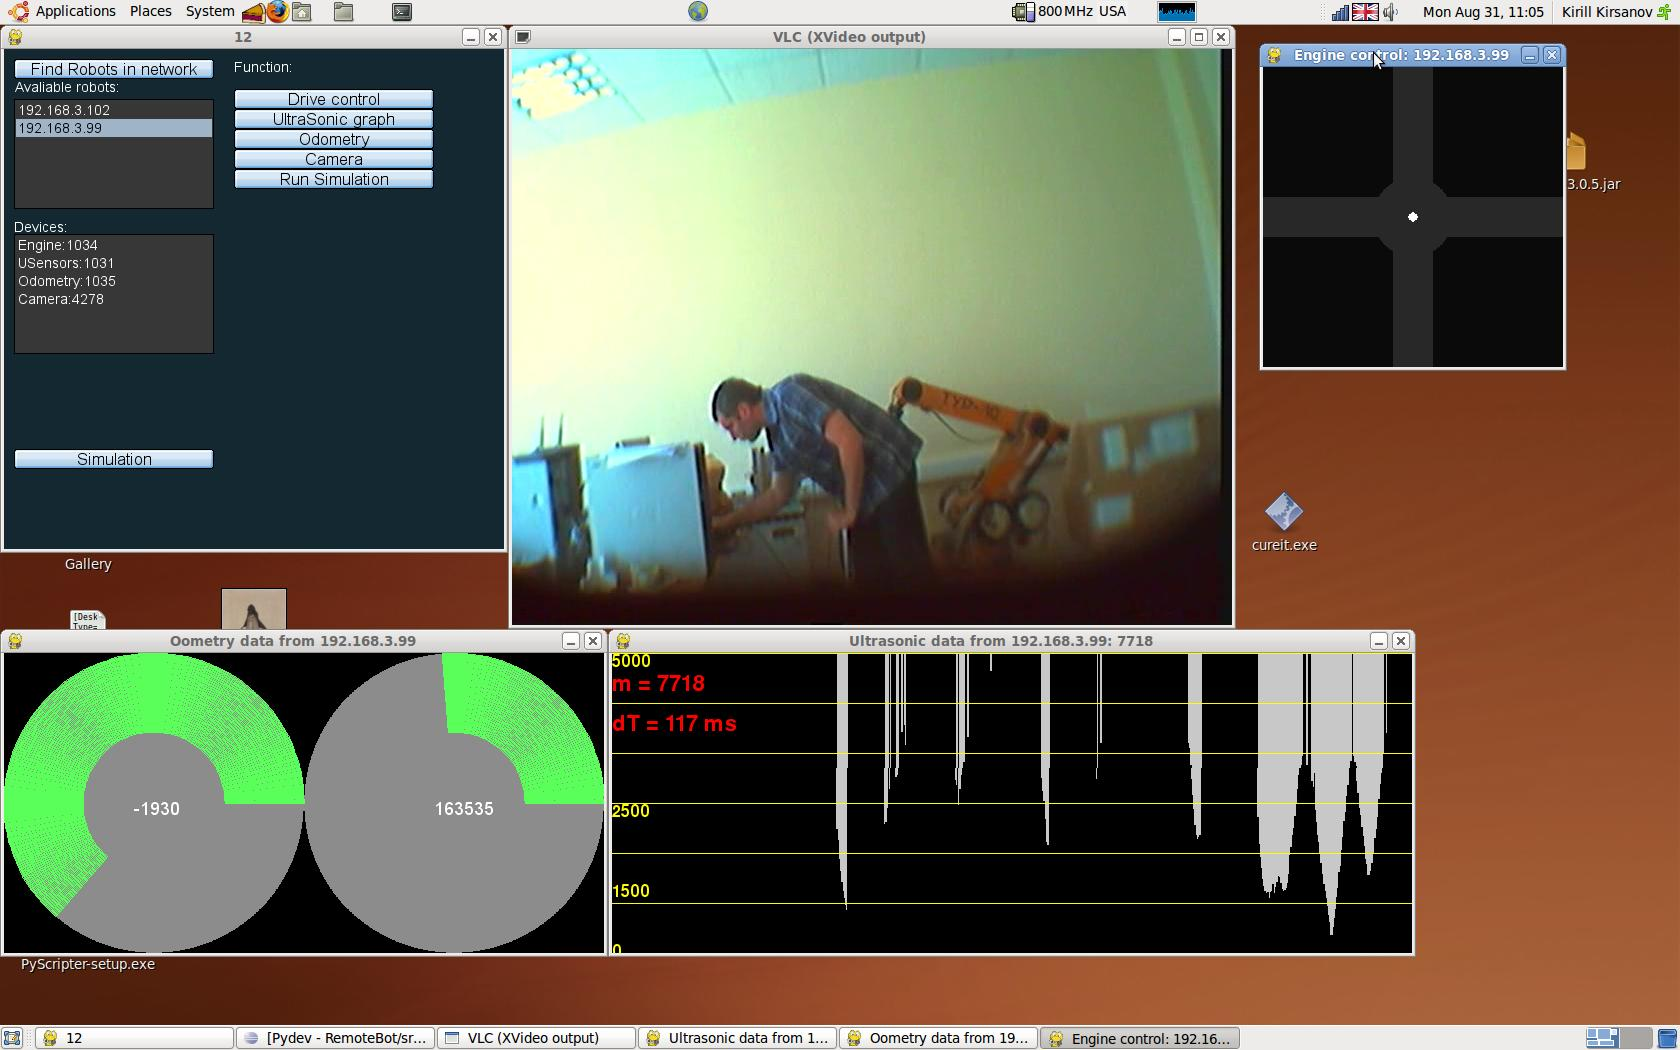
\includegraphics[width=3.2cm]{rob2.jpg}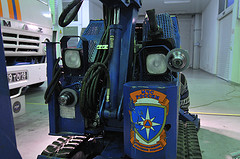
\includegraphics[width=3.2cm]{rob3.jpg}
\end{frame}

\begin{frame}
\frametitle{About field conditions\ldots}
%\framesubtitle{About field conditions\ldots}
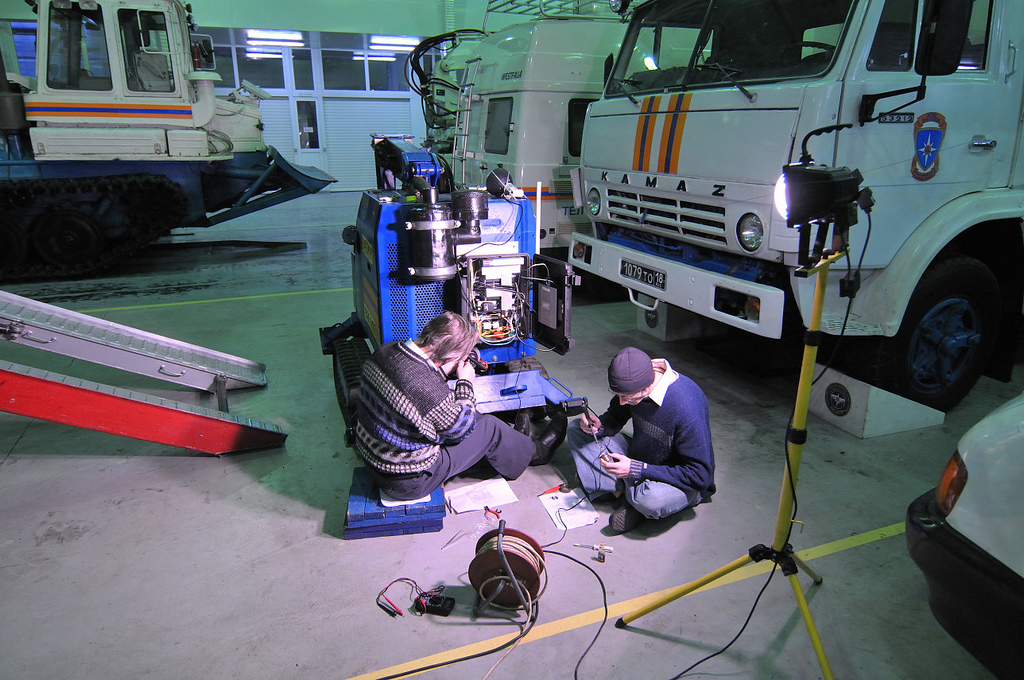
\includegraphics[width=11cm]{robot_big.jpg}
\end{frame}

\begin{frame}
\begin{center}
\begin{LARGE}
Questions?
\end{LARGE}
\end{center}
\footnotetext{How about raw perfomance? Why not LISP? Warkarounds for GIL?}
\end{frame}

\end{document}